\documentclass[a4paper, 12pt]{article}
\usepackage[a4paper,top=1.5cm, bottom=1.5cm, left=1cm, right=1cm]{geometry}

% Работа с русским языком
\usepackage[utf8]{inputenc}
\usepackage{mathtext}                % русские буквы в формулах
\usepackage[english, russian]{babel} % локализация и переносы

\usepackage{graphicx}   % Вставка изображений
\usepackage{float}      % "Плавающие" изображения3
\usepackage{wrapfig}    % Обтекание фигур (таблиц, картинок и прочего)
\usepackage{subfig}
\graphicspath{ {./images/} }

\usepackage{tabularx}
\usepackage{multirow}
\usepackage{booktabs}
\usepackage{amsmath}
\usepackage{amsfonts}
\usepackage{indentfirst}
\usepackage{longtable}
\usepackage{natbib}
\usepackage{bm}

\newcommand{\angstrom}{\text{\normalfont\AA}}
\newcommand{\e}[1]{\text{$\cdot10^{#1}$}}
\newcommand{\m}{\; м}
\newcommand{\mm}{\; мм}
\newcommand{\um}{\; мкм}
\newcommand{\A}{\; А}
\newcommand{\V}{\; В}
\newcommand{\uV}{\; мкВ}
\newcommand{\cels}{\; ^\circ С}

%%% Колонтитулы
\usepackage{titleps}
\newpagestyle{main}{
	\setheadrule{0.4pt}
	\sethead{Отчёт о выполнении лабораторной работы 2.2(2.3)}{}{}
	\setfootrule{0.4pt}                       
	\setfoot{ФРКТ МФТИ, 2024}{}{\thepage} 
}
\pagestyle{main}  

\begin{document}
    \begin{titlepage}
	\begin{center}
            {\large МОСКОВСКИЙ ФИЗИКО-ТЕХНИЧЕСКИЙ ИНСТИТУТ (НАЦИОНАЛЬНЫЙ ИССЛЕДОВАТЕЛЬСКИЙ УНИВЕРСИТЕТ)}
	\end{center}
 
	\begin{center}
		{\large Физтех-школа радиотехники и компьютерных технологий}
	\end{center}
	
	\vspace{8cm}
	{\LARGE
		\begin{center}
                {\bf Отчёт о выполнении лабораторной работы 2.2(2.3)}\\
                Изучение спектра атома водорода и молекулы йода
		\end{center}
	}
	\vspace{3 cm}
	\begin{flushright}
		{\Large Авторы: \\ 
        Тихонов Дмитрий Романович, \\ студент группы Б01-206а \\
        Павловский Кирилл Михайлович, \\ студент группы Б01-206а}
	\end{flushright}
	\vspace{4cm}
	\begin{center}
		\Large Долгопрудный, 2024
	\end{center}
    \end{titlepage}


    \section{Введение}

    \noindent \textbf{Цель работы:} исследовать сериальные закономерности в оптическом спектре водорода и спектр поглощения паров йода в видимой области. \\
	
    \noindent \textbf{В работе используются:} монохроматор УМ-2, коллиматор, неоновая лампа, ртутная лампа, водородная лампа, кювета с кристаллами йода, лампа накаливания на штативе.
    
    \section{Теоретическое введение}

    \subsection{Спектр возбужденных состояний молекулы}

    Изолированные атомы обладают дискретным спектром, который формируется из переходов электронов на более высокие энергетические уровни. В молекулах, в отличие от атомов, могут возбуждаться дополнительные степени свободы: колебательные и вращательные. В первом приближении, не учитывая взаимное влияние возбуждения электронов и дополнительных степеней свободы, получаем:

    \begin{equation}
        E = E_{\text{эл}} + E_{\text{колеб}} + E_{\text{вращат}},
    \end{equation}

    \begin{equation}
        \psi = \psi_{\text{эл}} \cdot \psi_{\text{колеб}} \cdot \psi_{\text{вращат}}.
    \end{equation}

    Таким образом, энергию молекулы можно рассматривать как отдельные компоненты, связанные с возбуждением электронов, колебаниями атомов в молекуле и вращением молекулы вокруг своих осей.

    \subsection{Масштабы составляющих энергии}

    \subsubsection{Электронные термы}

    Энергетические уровни молекул, -- \textit{термы}, связанные с переходами электронов, по происхождению идентичны электронным термам атомов.

    Характерная энергия электронных термов:
    \begin{equation}
        \hbar \omega_{\text{эл}} \approx R_y \sim 10 \text{ эВ}.
    \end{equation}

    \subsubsection{Энергия колебаний}

    Потенциал взаимодействия двух атомов представляет собой потенциальную яму с минимумом в точке $r_0$.

    \begin{figure}[H]
        \centering
        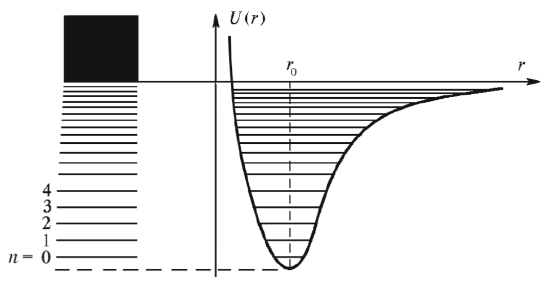
\includegraphics[width=0.6\linewidth]{images/ocsillation_levels.png}
        \caption{Схема энергетических уровней двухатомной молекулы}
        \label{fig:oscillation_levels}
    \end{figure}

    В молекуле могут возникать колебания атомов. Поскольку вблизи минимума потенциальная яма описывается параболой, нижние уровни энергии можно считать уровнями энергии гармонического осциллятора:
    \begin{equation}
        E_{\text{колеб}} = \hbar \omega_0 (n + \frac{1}{2}).
    \end{equation}

    Как можно видеть, уровни энергии являются равноотстоящими. При увеличении энергии начинает влиять \textit{ангармонизм} -- отступление от гармонического закона. Это приводит к изменению разностей энергии между уровнями.

    Оценим энергию колебаний. Будем считать, что при смещении на расстояние порядка боровского радиуса $a_0$ изменение потенциальной энергии составляет порядка $R_y$, тогда
    
    \begin{equation}
        U \sim \frac{(r - r_0)^2}{a_0^2} R_y + U(r_0) \quad \Rightarrow \quad k \sim \frac{R_y}{a_0^2}.
    \end{equation}
    
    Для частоты колебаний:
    
    \begin{equation}
        \omega_{\text{колеб}} = \sqrt{\frac{k}{M}} \sim \alpha^2 \frac{mc^2}{\hbar} \sqrt{\frac{m}{M}}.
    \end{equation}

    Сравним с электронными термами:
    \begin{equation}
        \omega_{\text{эл}} \sim \frac{R_y}{\hbar} \approx \alpha^2 \frac{mc^2}{\hbar} \quad \Rightarrow \quad \frac{E_{\text{колеб}}}{E_{\text{эл}}} \sim 10^{-3}.
    \end{equation}

    Таким образом, формируется расщепление электронных терм.

    \subsubsection{Энергия вращения}

    Каждая молекула имеет дискретный набор состояний, соответствующий вращению вокруг некоторой оси как целого. Оценим энергию этой степени свободы.

    \begin{equation}
        J = ma_0^2,
    \end{equation}

    где $J$ -- момент инерции относительно центра масс молекулы для оси, перпендикулярной оси молекулы.
    
    Энергия вращения квантуется:
    \begin{equation}
        E_{\text{вращ}} = \frac{\hbar^2}{2J} l(l+1).
    \end{equation}

    Сравнивая с электронными термами:
    \begin{equation}
        E_{\text{вращ}} \approx \frac{\hbar^2}{J} \approx \frac{\hbar^2}{Ma_0^2} \quad \Rightarrow \quad \frac{E_{\text{вращ}}}{E_{\text{эл}}} \approx \frac{m}{M},
    \end{equation}
    где $m$ -- масса электрона, $M$ -- масса молекулы.
    
    Итоговая оценка:
    \begin{equation}
        \omega_{\text{эл}} : \omega_{\text{колеб}} : \omega_{\text{вращ}} \sim 1 : \sqrt{\frac{m}{M}} : \frac{m}{M} \sim 1 : 10^{-3} : 10^{-6}.
        \label{eq:relation}
    \end{equation}

    \subsection{Наблюдаемые спектры}

    Оптические спектрометры работают в диапазонах энергий, соответствующим электронным термам ($E \sim 1$ эВ). Исходя из оценки  видно, что оптические спектрометры ($R \sim 1000$) не в состоянии наблюдать вращательные переходы. Таким образом, в полученных спектрах будут наблюдаться переходы между электронными уровнями, на которые наложены спектры колебательных степеней свободы.

    \begin{figure}[H]
        \centering
        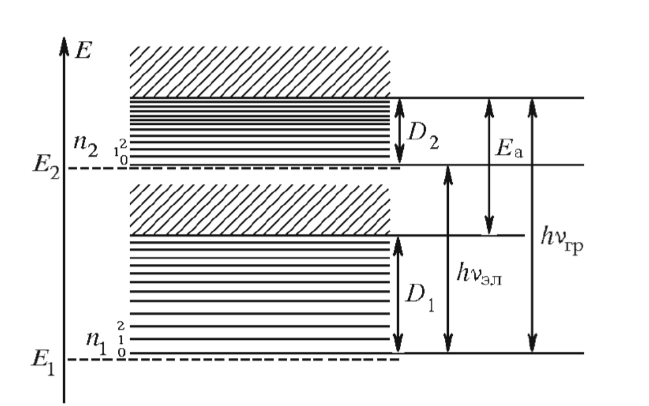
\includegraphics[width = 0.6\linewidth]{images/term_pair.png}
        \caption{Электронно-колебательные уровни двухатомной молекулы}
        \label{fig:term_pair}
    \end{figure}

    Штриховкой обозначен сплошной спектр, возникший из-за \textit{ангармонизма} потенциала. На рисунке также обозначены некоторые характерные энергии: $D_1, D_2$ -- энергии диссоциации для двух электронных терм, $h\nu_{\text{эл}}$ -- энергия электронного перехода, $E_a$ -- энергия возбуждения атома (переход из непрерывного спектра электронного терма 1 в непрерывный спектр электронного терма 2).

    Рассмотрим переходы молекулы йода $I_2$ в оптическом диапазоне. Все возможные переходы между колебательными уровнями соседних электронных состояний можно разбить на \textit{серии Деландра}.
    
    \begin{figure}[H]
        \centering
        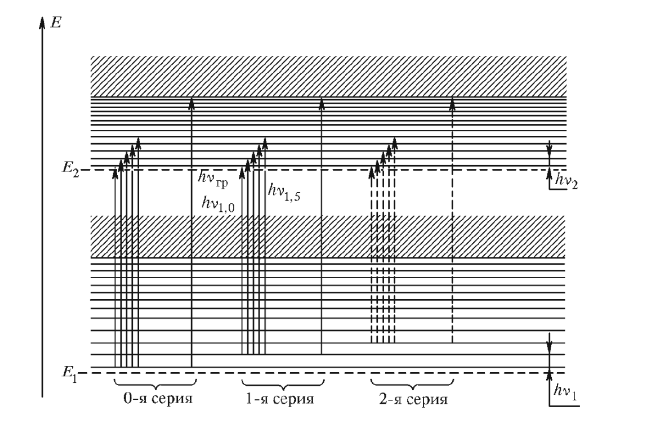
\includegraphics[width = 0.6\linewidth]{images/delandr_series.png}
        \caption{Электронно-колебательный спектр молекулы йода}
        \label{fig:delandr_series}
    \end{figure}
    
    Интенсивность каждой серии пропорциональна количеству частиц на колебательном уровне основного электронного состояния. В соответствии с распределением Больцмана получаем:

    $$
    N \sim e^{\frac{E}{kT}} \quad \Rightarrow \quad N_0 : N_1 : N_2 \approx 1 : \frac{1}{3} : \frac{1}{10}. 
    $$

    Энергетические положения линий:
    \begin{equation}
        h \nu_{0, n_2} = (E_2 - E_1) + h \nu_2 (n_2 + \frac{1}{2}) - \frac{1}{2} h \nu_1.
        \label{eq:lines}
    \end{equation}

    Очевидно, что расстояния между линиями будут равны $h \nu_2$. Следующая серия сдвинута в направлении меньших энергий на $h \nu_1$.

    В итоге мы получаем наложение нулевой и первой \textit{серий Деландра}.

    \begin{figure}[H]
        \centering
        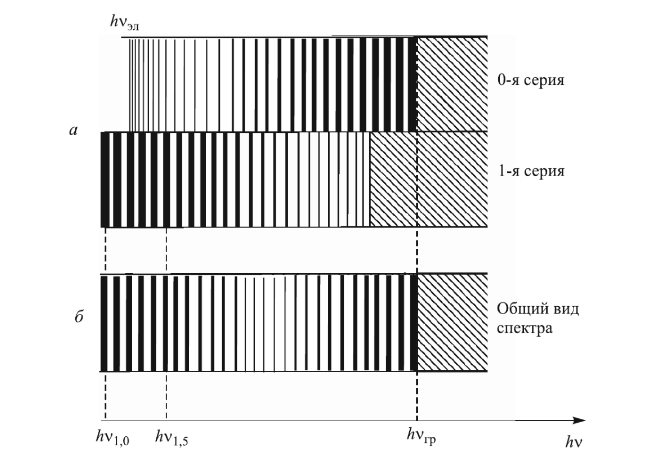
\includegraphics[width = 0.6\linewidth]{images/spectrum.png}
        \caption{Спектр поглощения паров йода}
        \label{fig:spectrum}
    \end{figure}

    \newpage
    
    \section{Методика измерений и экспериментальная установка}

    \begin{figure}[H]
        \centering
        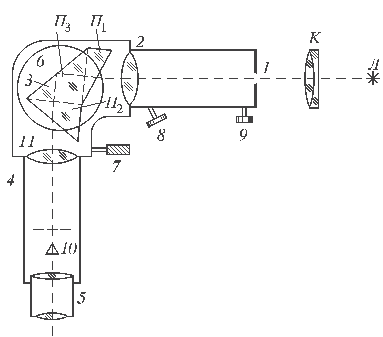
\includegraphics[width = 0.35\textwidth]{images/setup_1.pdf}
        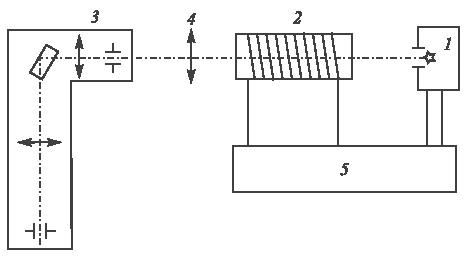
\includegraphics[width = 0.5\textwidth]{images/setup_2.pdf}
        \caption{Схема экспериментальной установки}
        \label{fig:exp_scheme}
    \end{figure}

    Для измерения длин волн спектральных линий в работе используется стеклянно-призменный монохроматор-спектрометр УМ-2 (универсальный монохроматор), предназначенный для спектральных исследований в диапазоне от $0.38$ до $1.00$ мкм.

    При подготовке УМ-2 к наблюдениям особое внимание следует обращать на тщательную фокусировку, с тем чтобы указатель 10 и спектральные линии имели чёткие, ясные границы. Фокусировка производится в следующем порядке. Перемещая окуляр, следует получить резкое изображение острия указателя 10. Осветив входную щель прибора ртутной лампой, нужно найти одну из спектральных линий и получить её резкое изображение при помощи микрометрического винта 8. При проведении измерений в другой части спектра, последняя операция по фокусировке должна проводиться вновь.
    
    Для отсчёта положения спектральной линии её центр совмещается с острием указателя. Отсчёт проводится по делениям барабана. Для уменьшения ошибки ширину входной щели делают по возможности малой ($0.05$ - $0.07$ мм по микрометрической шкале). Для наблюдения самых слабых линий в крайней фиолетовой области щель приходится несколько расширять. Глаз лучше замечает слабые линии в движении, поэтому при наблюдении полезно слегка поворачивать барабан в обе стороны от среднего положения.
    
    Спектрометр УМ-2 нуждается в предварительной градуировке. Для градуировки в коротковолновой части спектра удобно применять ртутную лампу ПРК-4, а в длинноволновой и средней части спектра -- неоновую лампу.

    В опытах по измерению длин волн бальмеровской серии источником света служит водородная трубка Н-образной формы, питаемая от источника высокого напряжения. Для увеличения яркости интересующих нас линий атомарного водорода в состав газа, которым заполняют трубку при её изготовлении, добавляют пары воды. Молекулы воды в электрическом разряде разлагаются, образуя атомарный водород. Следует отметить, что в спектре водородной лампы наряду с линиями атомного спектра наблюдается также спектр молекулярного водорода, интенсивность молекулярных линий которого значительно слабее.

    Молекулярный спектр поглощения паров йода можно наблюдать визуально на фоне сплошного спектра лампы накаливания 1, питаемой от блока питания 2 (рис. \ref{fig:exp_scheme} (справа)). Кювета 3 с кристаллами йода подогревается нихромовой спиралью, подключённой вместе с лампой накаливания к блоку питания. Линза 4 используется как конденсор. В результате подогрева кристаллы йода частично возгоняются, образуя пары с лёгкой фиолетовой окраской. Спектрометр позволяет визуально наблюдать линии поглощения молекул йода на фоне сплошного спектра излучения лампы накаливания видимой области (рис. \ref{fig:spectrum}).

    \newpage
	
    \section{Результаты измерений и обработка данных}
	
    Построим калибровочный график по спектрам неона и ртути (рис. \ref{fig:calibration_graph}).
    
    \begin{figure}[H]
        \centering
        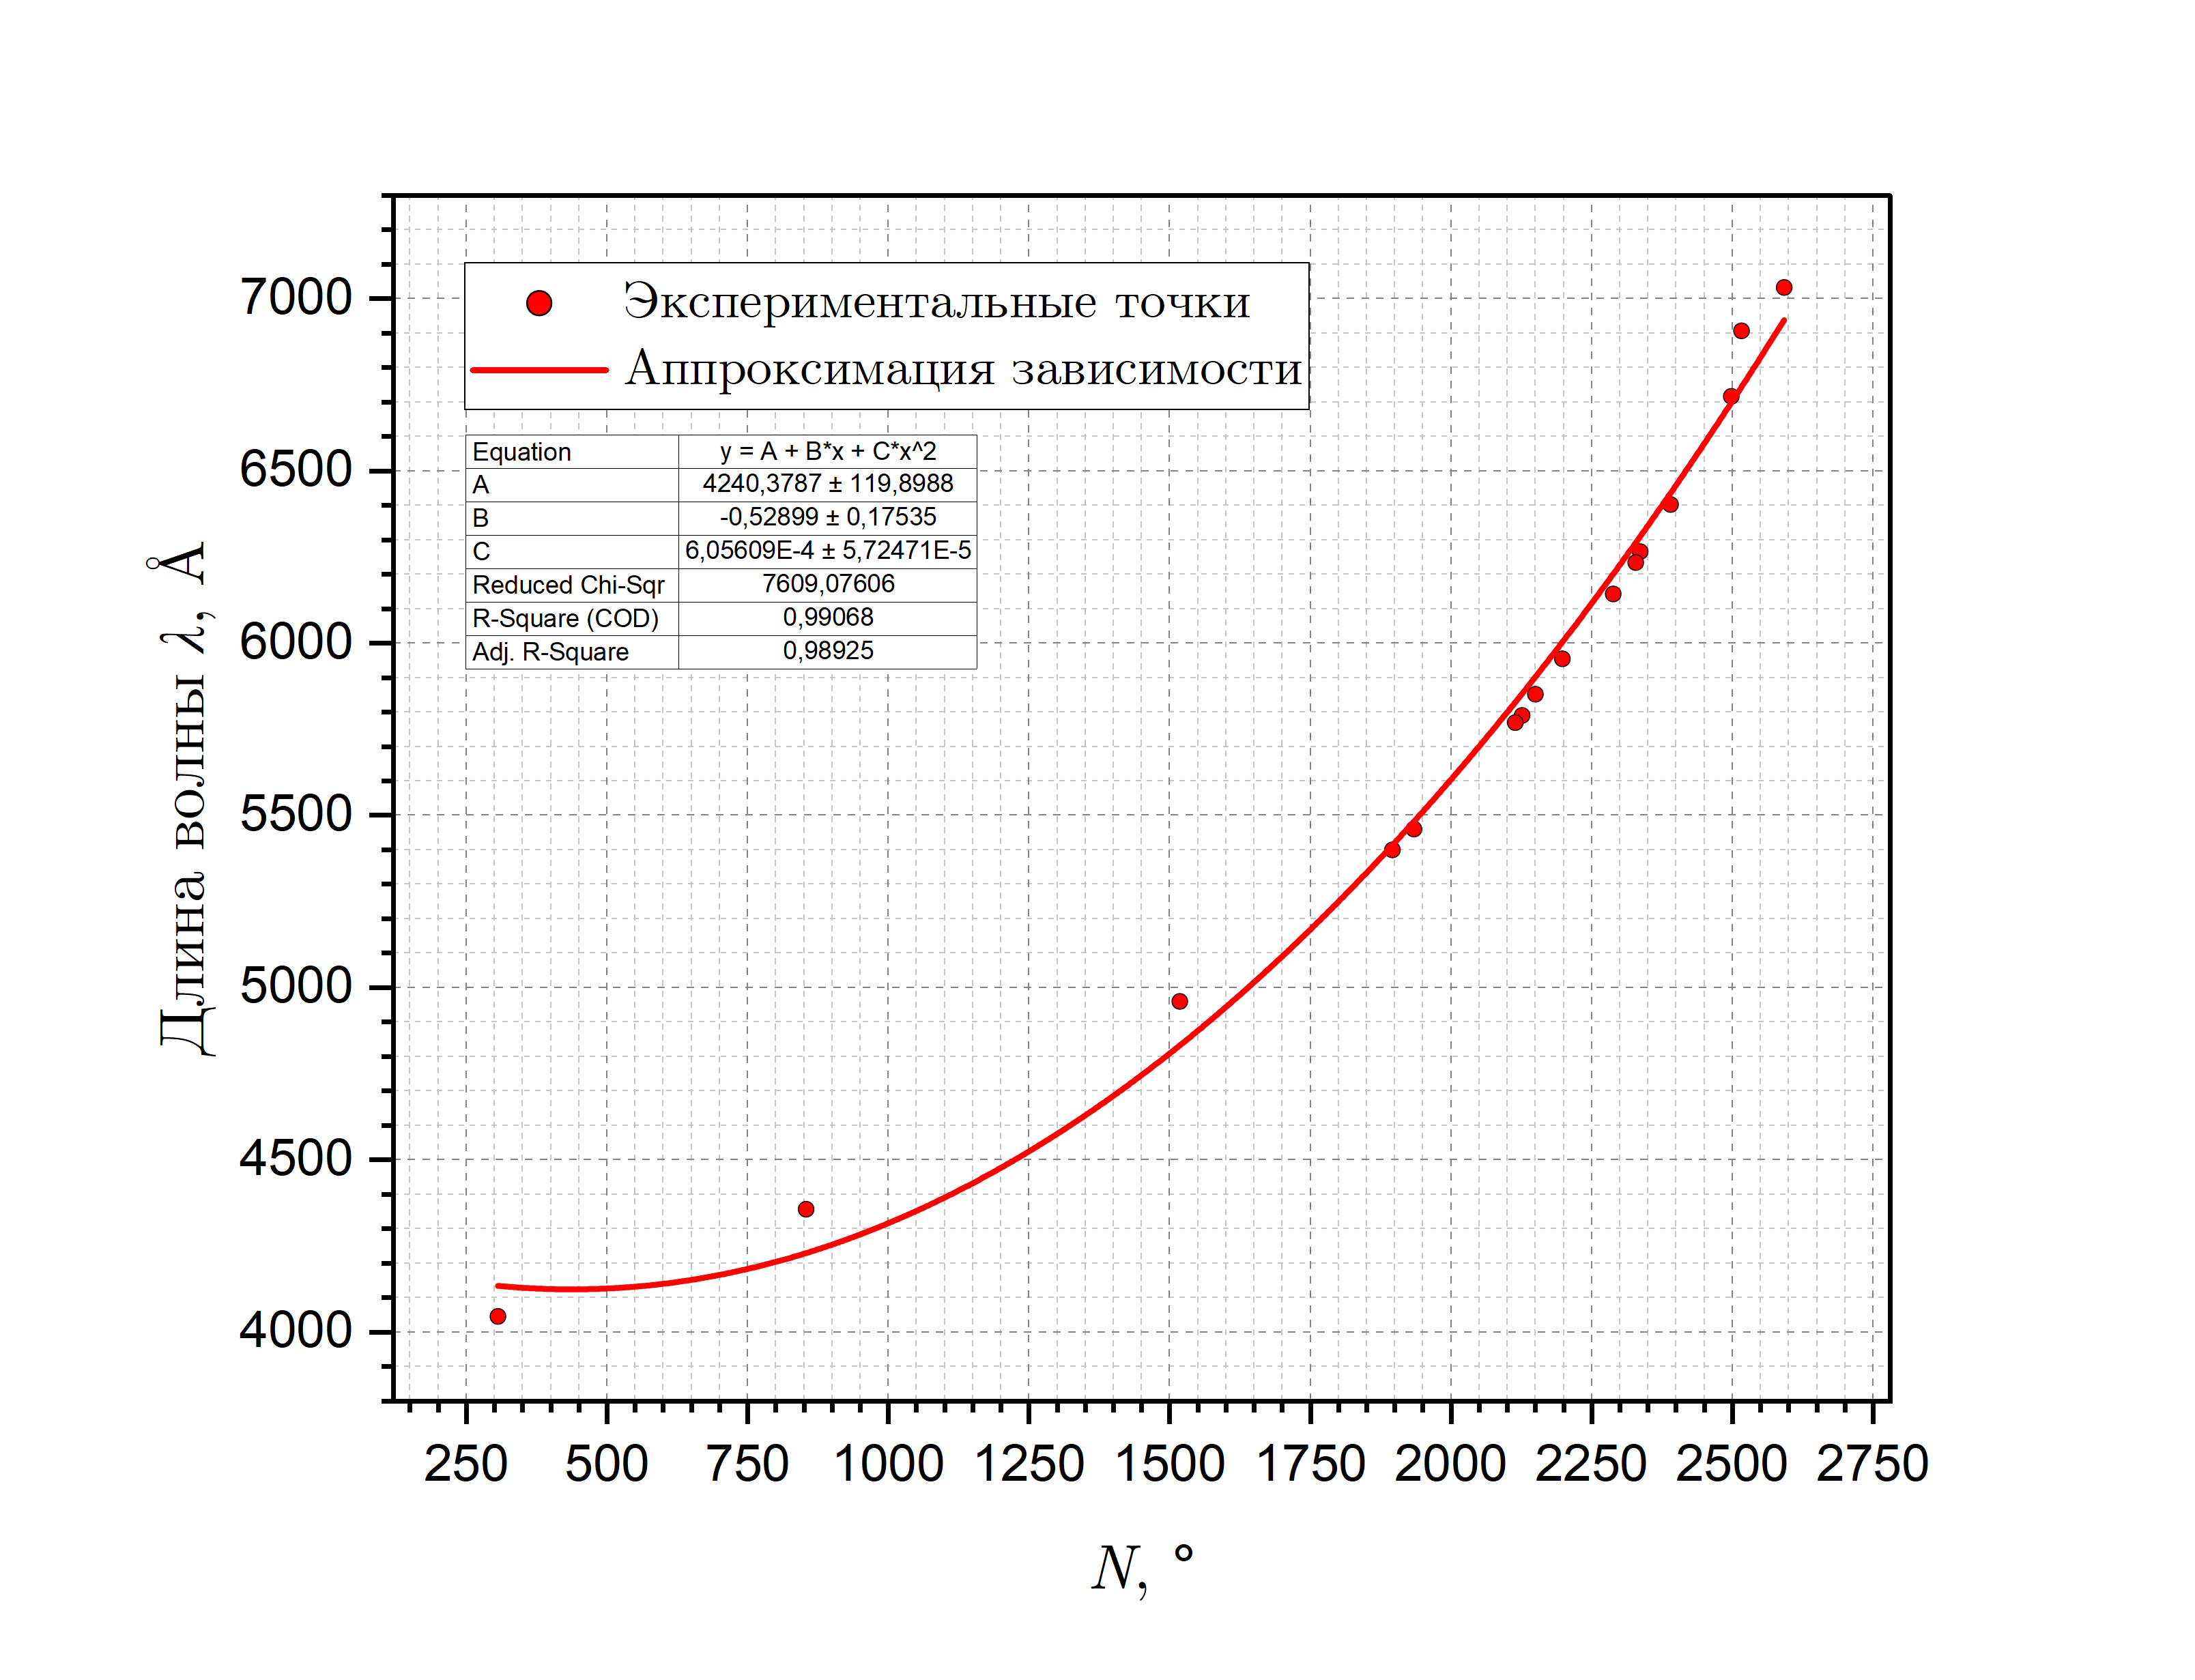
\includegraphics[width = 0.8\linewidth]{images/calibration_graph.png}
        \caption{Калибровочный график}
        \label{fig:calibration_graph}
    \end{figure}
    	
    Определим длины волн $H_\alpha$, $H_\beta$, $H_\gamma$, $H_\delta$ при помощи полученного калибровочного графика (рис. \ref{fig:calibration_graph}). Результаты приведены в таблице \ref{table:H}.
    
    \begin{table}[H]
        \centering
        \begin{tabular}{|c|c|c|c|c|}
            \hline
            & $N, ^\circ$ & $\sigma_N, ^\circ$ & $\lambda, \angstrom$ & $\sigma_\lambda, \angstrom$ \\ \hline
            $H_\alpha$  & $2448$ & $2$ & $6575$ & $200$ \\ \hline
            $H_\beta $  & $1464$ & $2$ & $4765$ & $135$ \\ \hline
            $H_\gamma$  & $1222$ & $2$ & $4500$ & $130$ \\ \hline
            $H_\delta$  & $828$  & $2$ & $4220$ & $120$ \\ \hline
        \end{tabular}
        \caption{Спектральные линии водорода}
        \label{table:H}
    \end{table}
    
    В пределах погрешности полученные значения совпадают с табличными для серии Бальмера. 
    
    Определим постоянную Ридберга. Длины волн спектральных линий водородоподобного атома описываются формулой
    $$
    \frac{1}{\lambda_{mn}} = Ry \cdot Z^2 \left( \frac{1}{n^2} - \frac{1}{m^2} \right)
    $$

    где $Ry$ -- константа, называемая постоянной Ридберга, $n = 2$ -- для серии Бальмера, величина $m$ для первых четырёх линий этой серии принимает значение 3, 4, 5, 6 ($H_\alpha$, $H_\beta$, $H_\gamma$, $H_\delta$).
    
    
    Построим график зависимости $ \lambda^{-1} $ от выражения вида $ 1/n^2 - 1/m^2 $ на рис.
    
    \begin{figure}[H]
        \centering
        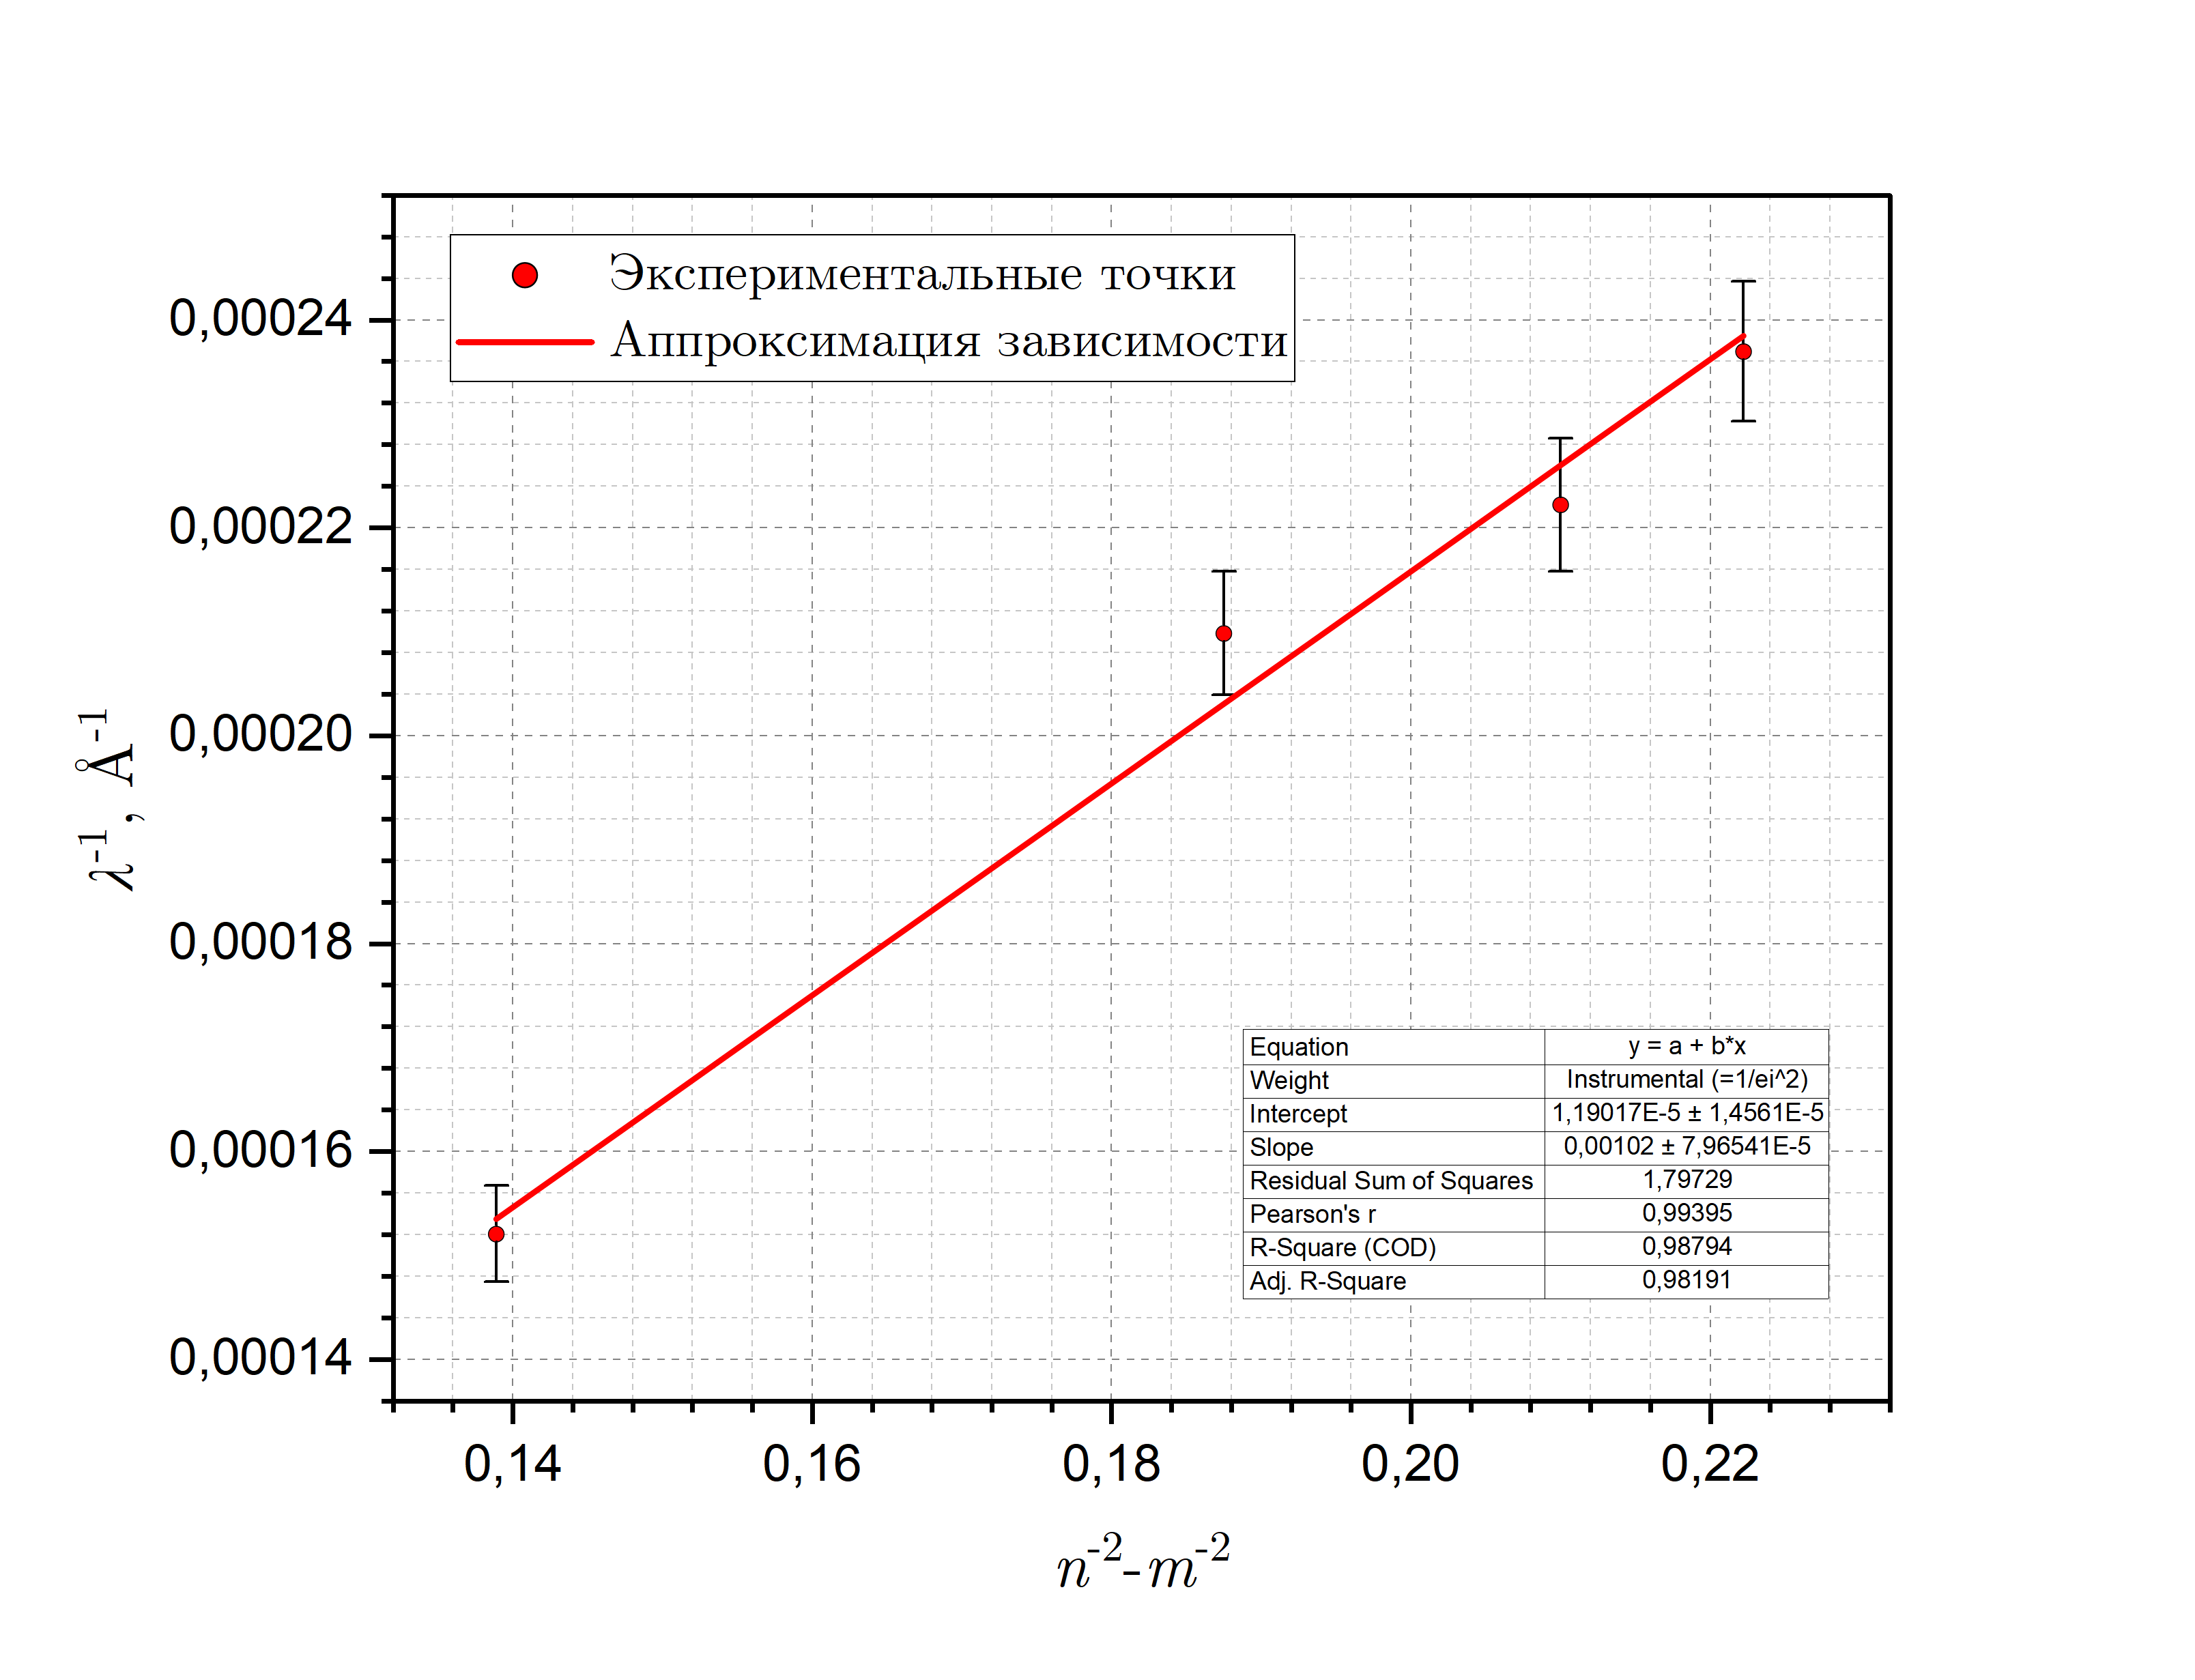
\includegraphics[width = 0.7\linewidth]{images/Ry_graph.png}
        \caption{Зависимость $ \lambda^{-1} $ от $ 1/2 - 1/m^2 $}
        \label{fig:graph3}
    \end{figure}
    
    Из графика видно, что $R = \left( 102 \pm 8 \right) \cdot 10^{3} \text{ см}^{-1}$. Это значение совпадает с табличным в пределах погрешности.
	
    Теперь определим длины волн линий поглощения для йода:
    
    \[\lambda_{1,0} = \left( 6.1 \pm 0.2 \right) \cdot 10^{3} \; \angstrom,\]
    \[\lambda_{1,5} = \left( 5.9 \pm 0.2 \right) \cdot 10^{3} \; \angstrom,\]
    \[\lambda_{гр}  = \left( 5.1 \pm 0.2 \right) \cdot 10^{3} \; \angstrom.\]
    
    Вычислим в электрон-вольтах энергию колебательного кванта возбуждённого состояния молекулы йода:
    
    \[h\nu_2 = \frac{h\nu_{1,5} - h\nu_{1,0}}{5} = \left( 0.0138 \pm 0.0005 \right) \text{ эВ}.\]
	
    Найдём параметры диссоциации молекул йода:
    \[h\nu_{эл} = h\nu_{1,0}+\dfrac{3}{2}h\nu_1 - \dfrac{1}{2}h\nu_2 = \left( 2.06 \pm 0.02 \right) \text{ эВ}, \]

    где $h\nu_1 = 0.027 \text{ эВ}$ -- энергия колебательного кванта основного состояния.
    
    Отсюда, энергии диссоциации частиц в основном и возбуждённом состояниях:
    
    \[D_1 = h\nu_{гр} - E_A       = \left( 1.50 \pm 0.02 \right) \text{ эВ},\]
    \[D_2 = h\nu_{гр} - h\nu_{эл} = \left( 0.38 \pm 0.02 \right) \text{ эВ},\]
    
    где $E_A = 0.94 \text{ эВ}$ -- энергия возбуждения атома.

    \newpage
    
    \section{Заключение}
    
    \begin{itemize}
        \item В данной работе были изучены спектры в оптических спектрах водорода и йода, экспериментально проверили справедливость формулы Бальмера.
        
        \item Была экспериментально определена постоянная Ридберга:
        $$
        \boxed{R_{\text{эксп}} = \left( 102 \pm 8 \right) \cdot 10^{3} \; \frac{1}{\text{cм}} \quad \left( R_{табл} = 109678 \; \frac{1}{\text{cм}} \right)}.
        $$
        \item Была получена энергия диссоциации частиц в возбуждённом и стабильном состоянии:

        $$
        \boxed{D_1 = \left( 1.50 \pm 0.02 \right) \text{ эВ}, \quad D_2 = \left( 0.38 \pm 0.02 \right) \text{ эВ}}.
        $$

        
    \end{itemize}
    
\end{document}